\documentclass[]{elsarticle} %review=doublespace preprint=single 5p=2 column
%%% Begin My package additions %%%%%%%%%%%%%%%%%%%
\usepackage[hyphens]{url}

  \journal{Forest Ecology and Management} % Sets Journal name


\usepackage{lineno} % add
\providecommand{\tightlist}{%
  \setlength{\itemsep}{0pt}\setlength{\parskip}{0pt}}

\usepackage{graphicx}
\usepackage{booktabs} % book-quality tables
%%%%%%%%%%%%%%%% end my additions to header

\usepackage[T1]{fontenc}
\usepackage{lmodern}
\usepackage{amssymb,amsmath}
\usepackage{ifxetex,ifluatex}
\usepackage{fixltx2e} % provides \textsubscript
% use upquote if available, for straight quotes in verbatim environments
\IfFileExists{upquote.sty}{\usepackage{upquote}}{}
\ifnum 0\ifxetex 1\fi\ifluatex 1\fi=0 % if pdftex
  \usepackage[utf8]{inputenc}
\else % if luatex or xelatex
  \usepackage{fontspec}
  \ifxetex
    \usepackage{xltxtra,xunicode}
  \fi
  \defaultfontfeatures{Mapping=tex-text,Scale=MatchLowercase}
  \newcommand{\euro}{€}
\fi
% use microtype if available
\IfFileExists{microtype.sty}{\usepackage{microtype}}{}
\bibliographystyle{elsarticle-harv}
\usepackage{longtable}
\usepackage{graphicx}
\ifxetex
  \usepackage[setpagesize=false, % page size defined by xetex
              unicode=false, % unicode breaks when used with xetex
              xetex]{hyperref}
\else
  \usepackage[unicode=true]{hyperref}
\fi
\hypersetup{breaklinks=true,
            bookmarks=true,
            pdfauthor={},
            pdftitle={Interpreting wind damage - How management impacts standing timber at risk of wind felling},
            colorlinks=false,
            urlcolor=blue,
            linkcolor=magenta,
            pdfborder={0 0 0}}
\urlstyle{same}  % don't use monospace font for urls

\setcounter{secnumdepth}{5}
% Pandoc toggle for numbering sections (defaults to be off)


% Pandoc header



\begin{document}
\begin{frontmatter}

  \title{Interpreting wind damage - How management impacts standing timber at risk of wind felling}
    \author[Department of Biological and Environmental Science]{Mária Potterf\corref{1}}
   \ead{mpotterf@jyu.fi} 
    \author[Department of Biological and Environmental Science]{Kyle Eyvindson}
   \ead{kyle.j.eyvindson@jyu.fi} 
    \author[Department of Biological and Environmental Science]{Clemens Blattert}
   \ead{clemens.c.blattert@jyu.fi} 
    \author[Department of Biological and Environmental Science]{Daniel Burgas}
   \ead{daniel.d.burgas-riera@jyu.fi} 
    \author[Department of Biological and Environmental Science]{Mikko Mönkkönen}
   \ead{mikko.monkkonen@jyu.fi} 
      \address[University of Jyvaskyla]{Department of Biological and Environmental Science, University of Jyvaskyla, P.O. Box 35, FI-40014 Jyvaskyla, Finland}
    \address[Wisdom]{This is wisdom address}
    \address[LUKE]{THIS is Luke address Department, Street, City, State, Zip}
      \cortext[1]{Corresponding Author}
    \cortext[]{}
  
  \begin{abstract}
  Novel forest management strategies such as new harvesting methods, landscape-level optimization, or diversification of harvest intensity over the landscape (including setting stands aside) promisingly balance between economic and ecologic objectives of forested landscapes. Yet, it remains unclear how those will shape stand susceptibility to natural disturbances such as windthrows. We hypothesize that 1) harvesting methods promoting continuous tree cover will increase risk of wind damage, and 2) higher volume of standing trees will increase wind damage risk.
  
  Here, we simulated the development of 1470 forest stands in Central Finland under various rotation (RF), continuous cover forestry (CCF) and set-aside (SA, no management) regimes over 100 years. We optimized the management regimes to obtain an even flow of timber while maximizing the regions multifunctionality (combining provision of non-woody ecosystem services and endangered species habitats). We defined a range of landscape-level harvest intensity scenarios from completely SA landscapes (no income) to highest even flow timber, where actively managed stands were exclusively under RF or CCF regimes. We calculated the wind damage risk for each stand and scenario using a generalized linear model (Suvanto et al., 2019). We investigated how the increasing harvesting intensity will affect mean wind risk (\%) and standing top stratum timber volume (m3) at alternative scenarios.
  
  Mean probability of wind damage slightly increased (CCF) or remained nearly constant (RF) with increasing harvest intensities. Stands under active RF had half of the wind risk probability compared to stands under CCF; wind risk of SA stands decreased with increasing harvest intensities (Figure 1A). Standing top stratum volume accumulated in SA stands within both CCF and RF landscapes and decreased with increasing harvest intensities. Top stratum timber volume was approximately 50\% higher in RF (µ=\textasciitilde150 m3) compared to landscape managed solely by CCF (µ=\textasciitilde100 m3), especially at low harvest intensity (Figure 1B).
  
  We conclude that when interpreting the risk of wind damage among management regimes, we need to take into account the standing timber volume exposed to risk in order to understand the potential economic loses.
  \end{abstract}
  
 \end{frontmatter}

\newpage

\hypertarget{introduction}{%
\section{Introduction}\label{introduction}}

Importance of increasing disturbances and associated timber damage

Disturbances and climate change associated stand level damage will increase on global nad local scales.

Novel managements seeks for balance between economy and ecology

Novel methos of the forest managements balances between provision of timber, non-woody ecosystem services by optimazing the harvesting priorities given equal weights to timber, non-woody ESS and deadwood associated biodiversity. These novel methods implements wider options for management regimes within rotation forestry including thining, non wthinning or increading number of retained green trees after the final cut, or developting new harvesting methods such as continuous cover forests that seems t promisingly balance between simultaneous provision of timber and non-woody ecosystem services.

Landscape level management combine the approaches to balance economy-ecology

LAndscape level scale for management planing, along with optimization for specific targets aiming to non-timber benefits along to it monetary values allows to allocate the most beneficail managenet regimes based on initial stand condition and state and potential of whole groups of stands to generate required values over whole landscape. THis approach can on one hand dedicate the stand to completely set aside regime to shelter biodiversity and on another hand increase harvesting levels on separated stands, creating a landscape level mosaic of various management regimes applied over the alternative landscape. Both approaches have however consequences of subseuqnet wind risk of individual and their neighboring stands.

What managements are done to reduce wind risk?

Multiple management regimes aim to reduce the risk of wind damage for example by reducing rotation age Zimová et al. (2020)

The forest management needs to simultaneously deliver timber, non-woody ecosystem services and shalter biodiveristy under constant threat of increasing disturbances. frequencies or simply by changing climatic conditions that e.g.~exposes trees to wind damage by lowering tree anchorage during the windiest time of the year.

The frequency of teh climatic disruptions will increase and as such will increase teh potential damage t individual stands and the

Novel methods of teh forest management are needed to

Future forest ecosystems need to simultaneously provide timber, non-woody ecosystem services such as carbon storage or human recreation, and shelter biodiversity.\\
To balance between biodiversity and timber economic gains, the proportion of set-aside forests within commercial forests emerges, and new forest management approaches are explored, such as continuous forest cover (Eyvindson et al., 2021) and traditional harvesting regimes are becoming controversial or requested to ban (\ldots). The increase of the set aside forests within the commercial forests, as well as development of the new management techniques affect landscape level structural diversity, timing of the thinning, presence of absence of the final cuts in rotation forestry or development of the larger trees within continuous cover forestry or in set-aside forestry. The fundamental is the carefull landscape level planning of the management actions balancing between set-aside (unmanaged forests), intensive management and continuously present forest cover.

Optimal management scenarios fullfil the specific objectives of the society of forest owners to provide certain timber value, improve provision of timber and non-timber ecosystem services, or improve overall forest multifunctionality of the landscape. As such, optimization provides the combination of the specific forest management regimes on stand level. Althought the optimization process does not necessary involve the spatial configuration of the stands, it specifically assigns the particular regimes to individual stands and therefore allows to recreate alternative dynamics landscapes shaped by forest managements aggregated by optimal scenarios. As such, the spatial configuration of the management regimes allows to estimate the subsequent characteristics such as landscape level risk of wind damage.

The risk of the wind damage increases with current climate change and it creates the major risk to the stability of the forest production. Windthrows are unpredictable climatic disruption that shapes forest structure and composition, and if left unsalvaged could create opportiunities for deadwood dependent species and support local biodiversity. From economical point of view, however, windthrows massively abrupt the continuity of the timber supply, lowers timber quality from log to pulp, increases the prices of unplanned salvage harvesting (REF). To lower the risk of wind risk damage, current suggestions include shortening the rotation period, promoting/avoiding the wind resistant vs.~wind prone tree specuies, advocate for shortening of the minimal stand age (Latvia REF). This however poses further pressure on the multifucntionnal and multiple objective oriented landscapes, which will provide habitats for endangered species, support non-timber services and forest recreational use.

Traditional forest management regimes specialized in promoting timber revenues while minimizing costs. In Fennoscandia, over the decades, the traditional rotation forestry with multiple thinnings and final cuts that over just mutlipel decades (from 1950) homogenized stands structureal diversity, homogenized landscapes and increased forest fragmenetations. On the other hand, forest management supporting multifunctional landscapes, and promoting non-timber ecosystem services requires implementation of the diverse set of management regimes (Mönkkönen et al., 2014; Triviño et al., 2017). Furthermore, provision of the endangered species habitats and non-woody ecosystem services are provided on different scales where the planning scale should match or overcome the scale that provided ecosystem (Pohjanmies et al., 2019).

Here we explore how the restriction of forest management practices, along with the increasing level of harvest levels over the landscape affects landscape level damage of wind risk and how much timber value is put on risk under alternative regimes and extraction levels. Our study for the first time evaluates the landcspeca level wind risk combined with the forest growth simulator and long-term consequences of he applied forest management practices. Therefore, we first calculate the stand level wind risk over alternative landscapes and further explore the likely drivers of the wind risk levels. We investigated how restriction of forest management regimes combined with levels of intensity of timber extraction will affects landscape level wind risk.

Our study aims to understand how types of forest management and harvesting intensity affect stand and landcape level wind risk over time, and how much timber volume is at the risk at time. We hypothetized that RF will increase stand level wind risk due accumulated timber volume before the final cut, and increase wind risk in landscape due to increasing number of stands with open edges after the final cuts. On the other hand, the CCF will likely homogenize the amount of timber volume over landscape; therefore at any given time, the exposed timber volume to wind damage will be lower in CCF compared to RF management. We wil consider the pulp and log volume of the standing volume. We futher investigate the dynamics of simulated stand characteristics as stand dominant height, dominant tree speciecs by stand, age, number of trees by stand, frequency of opend edge stands and thinning frequency over the landscape over the harvest intensity gradient and time. We further differentiate between the dynamics of the volume and wind risk in managed and set-aside forests.

(Triviño et al., 2017) no single management alone is able to balance timber and biodiversity demand, and we need to combine management regimes over the landscape to balance between nonw-woody ESS, biodiversity and timber production. WE need to diversity forest management over the landscape to support multifunctionnality (Triviño et al., 2017)

Althought the larger spatial planning scale improves a little bit the mitigation between economic and ecological benefits, the succesful restoration of deadwood dependent biodiversity will likely require active deadwod creation (Pohjanmies et al., 2019).

CCF is a cost-efficient tool to increase multifunctionnality in fennoscandia (Peura et al., 2018)

\hypertarget{methods}{%
\section{Methods}\label{methods}}

\hypertarget{study-area}{%
\subsection{Study area}\label{study-area}}

Our study area represents a typical Finnish production forested landscape with relatively structurally homogenous forests stands. In total, we used 1470 forests stands aggregated within a single watershed (number 14.534) in Central Finland, covering 2242 ha (Fig. \ref{study_area}). Initial stand conditions were collected as open source data from the Finnish Forest Centre (available on www.metsaan.fi) providing currents stand conditions in 2016.

\begin{figure}
\centering
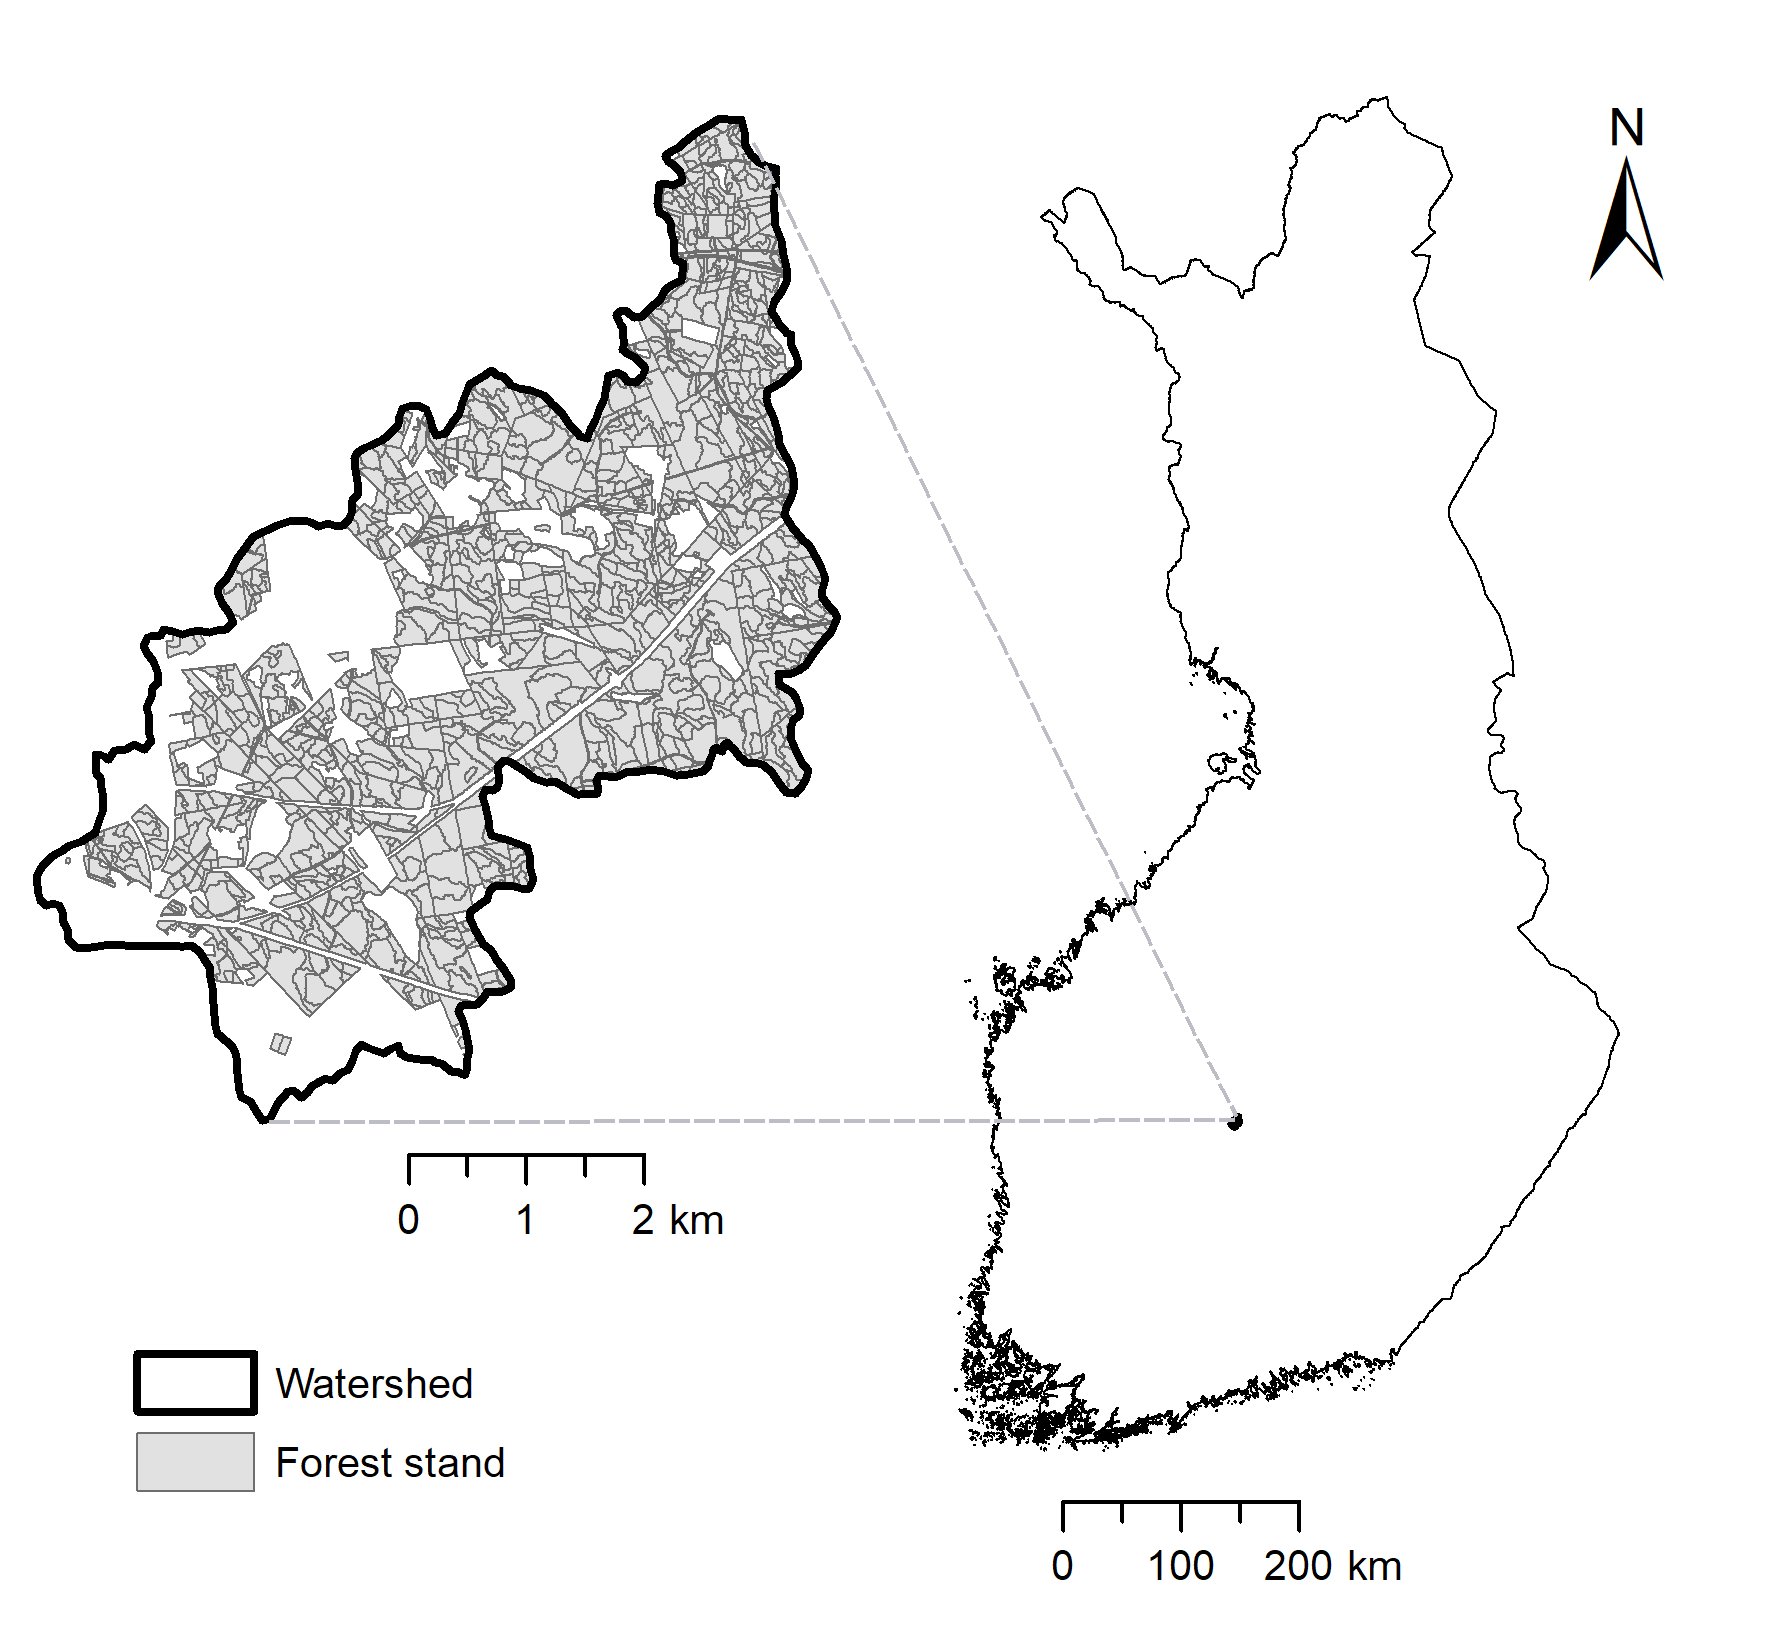
\includegraphics{/projappl/project_2003256/windDamage/externalFigs/studyArea_crop.png}
\caption{The study area located in Central Finland (watershed 14.534) comprising 1475 forest stands.\label{study_area}}
\end{figure}

Our input dataset included initial stand conditions (2016). We simulated the alternative development of individual forest stands under the various forest management regimes over 100 years. We have optimized the management regimes over the landscape to create a harvest intensity gradient varying from completely set aside landscape (no income) to highest even-flow timber and multifunctionnality. For each stand, scenario and year, we have calculated wind damage risk. We further interpreted wind risk in terms of standing log and pulp top layer timber given active or set aside management, landscape level scenario and time (Fig. \ref{workflow}). We processed the datasets, calculated damage probability models, and visualized results using R Development Core Team (2019).

\begin{figure}
\centering
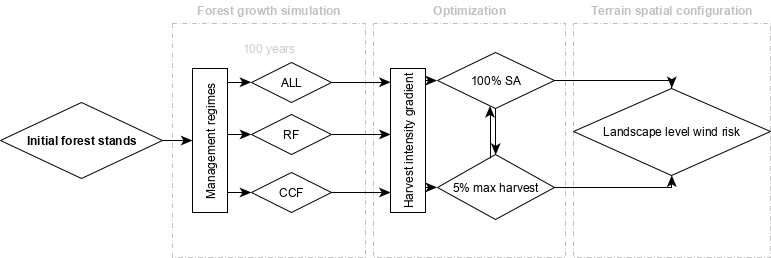
\includegraphics{/projappl/project_2003256/windDamage/externalFigs/overview2_horizontal.png}
\caption{The study workflow from collecting initial stand conditions (2016) throught forest simulation growth under alternative management regimes, landscape-level optimization and to construct harvest intensity gradient \label{workflow}}
\end{figure}

\hypertarget{forest-stand-development-under-different-regimes}{%
\subsection{Forest stand development under different regimes}\label{forest-stand-development-under-different-regimes}}

We simulated the development of the forests stands using SIMO forest growth simulator (Rasinmäki et al., 2009) over 100 years, separated into 20 5-year sequences. Each stand could be managed by up to 58 different management regimes (the total number of regimes per stands depended on the initial stand conditions), including 17 regimes for rotation forestry (RF), 40 variations of continuous cover forest (CCF) and one set-aside (SA), where no management actions were taken. RF regimes differed in timing of final felling, optional thinning (present/absent), and increase in number of retained green trees after final cut (more details in Eyvindson and Kangas (2018)). Basic CCF management follows rules from Äijälä et al. (2014). To increase the range of CCF managements, we varied two rules defining the timing of harvest: (i) site-specific basal area and (ii) timing of the first thinning. We modified the pre-defined site-specific basal area requirement (16m2/ha for less fertile sites to 22m2/ha for fertile sites) prior to harvesting by -3, ±0, +3, +6, and delayed the timing of the first harvest in 5 year increments up to a delay of 45 years.

\hypertarget{optimization}{%
\subsection{Optimization}\label{optimization}}

The optimization balances between harvest intensity (net present income, NPI) and landscape-level multifunctionnality, including non-woody ecosystem services (climate change mitigation), recreational activities and vertebrate and non-vertebrate endangered species. NPI represents economic value of the forests estimated by Metsähallitus (the Finnish governmental organization managing state owned forests). Landscape level optimization creates alternative landscapes varying over harvest intensity gradient. Specifically, this varies from completely SA landscape (all stands are SA, NPI=0) to highest NPI values (leaving at most 5\% of stands under SA). We run three optimizations: using exclusively RF, CCF, or both RF and CCF allowed (further reffered as ALL).
The optimization resulted in 63 alternative landscapes for RF, CCF and ALL manamement regimes over the harvest intensity gradient, where each landscape contained stands under RF, CCF or SA regimes. The share of SA over landscape increased with decreasing NPI values.

\hypertarget{wind-risk-calculation}{%
\subsection{Wind risk calculation}\label{wind-risk-calculation}}

We have calculated the probability of wind damage based on Suvanto et al. (2019) binomial generalized linear model with logit-link function for each stand for every time step at each scenario. Suvanto et al. (2019) model calculates the probability of the wind damage considering available relevant open-access datasets including dominant tree species, dominant tree height, time since thinning, predicted levels on maximal wind speed, temperature sums, evaluated if stand has open edge, soil type, mineral soil depth, site fertility and temperature sum (see Suvanto et al. (2019) for all details). The final probability of wind damage shows relative differences between stands, whereas the damage can be only partial to the stand, but neglects the explicit spatial locations of the future strongs winds. The parameters of the dominant tree species, tree height, open edge and time since thinning were dynamics under simulated management regimes. Parameters of maximal predicted wind speed and temperature sums, as well as soil characteristics, remained stable during our 100 years simulation.

\hypertarget{data-processing}{%
\subsection{Data processing}\label{data-processing}}

We calculated the probability of wind damage for each stand, scenario and time. Further, we averaged the wind risk values over the scenarios to allow comparison between RF, CCF and ALL management regimes groups over the harvest gradient. We explored the mean wind risk (\%) for each scenario, harvest gradient (from set-aside to maximal harvest levels) and between stands under active (RF, CCF, ALL) or set-aside management. In addition, we investigated the mean volume of standing log and pulp timber (m3) for scenarios and harvest gradient and over time.

\hypertarget{results}{%
\section{Results}\label{results}}

\hypertarget{mean-wind-risk-over-npi-and-time}{%
\subsection{Mean wind risk over NPI and time}\label{mean-wind-risk-over-npi-and-time}}

The mean wind risk damage was higher for landscapes managed by CCF that for landscapes managed exclusively by RF. Tt remained relatively stable over harvest intensity gradient for activelly managed stands, but was two times higher in stands under CCF than RF management (Fig. @ref(fig:mean\_risk\_NPI\_time A)). Mean wind damage risk decreased in Set Aside stands with increasing harvest intensity. Over time, the wind risk trippled over 100 year for stands under CCF regimes and remained constant (\textasciitilde0.02) for RF managed stands. In SA stands, wthe wind risks slightly increased (Fig. XXX B).

\begin{figure}
\centering
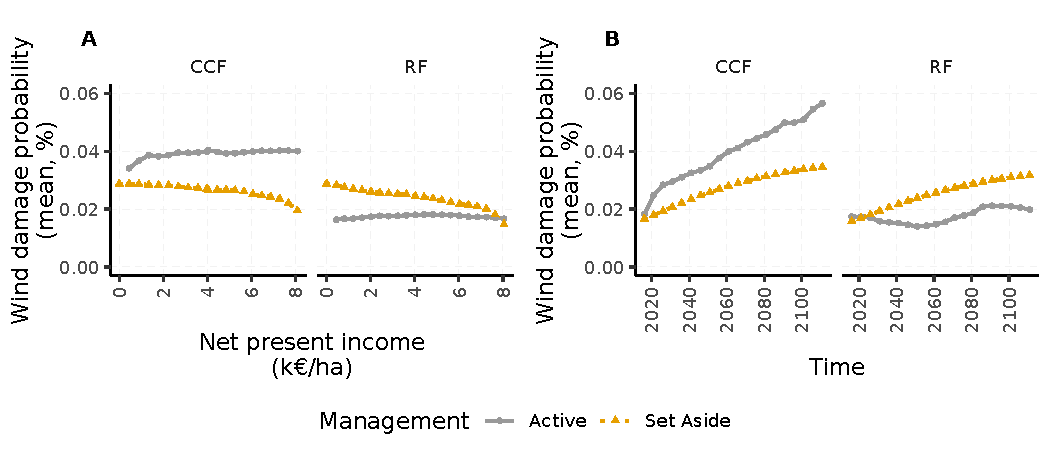
\includegraphics{test_manus4_puhti_files/figure-latex/mean_risk_NPI_time-1.pdf}
\caption{(\#fig:mean\_risk\_NPI\_time)Mean wind damage probability over A) harvest intensity gradient (net present income) and B) time for alternative management landscapes including stands under active (continuous cover (CCF) and rotation forestry (RF)) and set aside (SA) regime.}
\end{figure}

\hypertarget{top-layer-standing-timber-at-risk}{%
\subsection{Top layer standing timber at risk}\label{top-layer-standing-timber-at-risk}}

Mean standing timber log volume in SA stands decreases with increasing harvest intensity gradien (Fig. XXX A) and increases over time (Fig. XXX B). In both landscape management regimes remines relatively stable with increasing harvest intensity (\textasciitilde60 m3/ha) while slightly increases over years in CCF or decreases in RF (Fig. XXX B). Large differences in standing timber volume are howerever visible in standing pulp timber: the standing pulp wood almost triples (100 m3 to 30 m\^{}3/ha for RF and CCF, respectivelly) the standing pulp volume in CCF managed stands. Compared to SA management, CCF reduces the amount of pulp timber over whole harvest intensity gradient, and specifficaly after 20 years of first CCF application (from 2040, Fig. XXX D). On the other hand, RF increases the proportion of pulp timber in expenses of log volume over time.

\begin{figure}
\centering
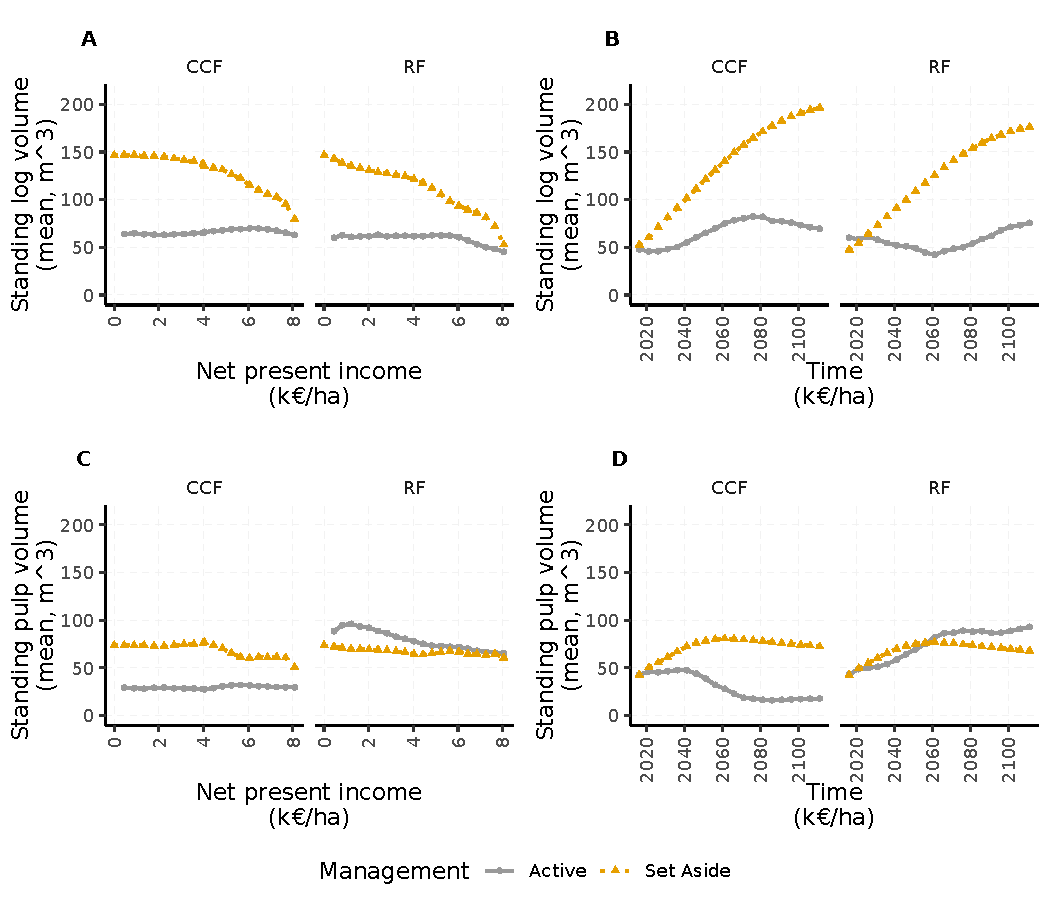
\includegraphics{test_manus4_puhti_files/figure-latex/mean_V_NPI_time-1.pdf}
\caption{(\#fig:mean\_V\_NPI\_time)Mean standing log (upper row, A, B) and pulp (lower row, C, D) timber volume over harvest intensity gradient (left, A,C) and time (right, B, D) for alternative management landscapes including stands under active (continuous cover (CCF) and rotation forestry (RF)) or set aside (SA) regime.}
\end{figure}

\hypertarget{discussion}{%
\section{Discussion}\label{discussion}}

\hypertarget{wind-risk-dynamics}{%
\subsubsection{Wind risk dynamics}\label{wind-risk-dynamics}}

We found that intensification of the harvesting regimes have different conseuqences of resulting wind risk: where CCF management increases wind risk, and RF lowers wind risk with increasing intensity.

\hypertarget{wind-risk-drivers}{%
\subsubsection{Wind risk drivers}\label{wind-risk-drivers}}

\hypertarget{future-questions-to-answer}{%
\subsubsection{Future questions to answer}\label{future-questions-to-answer}}

\hypertarget{recommendation-for-future-management}{%
\subsubsection{Recommendation for future management}\label{recommendation-for-future-management}}

\begin{itemize}
\tightlist
\item
  SA vs.~intensification of management
\item
  management types: CCF, RF or ALL or something else???
\end{itemize}

Wind (10 years return level of max wind speed REF) are estimated the same over 100 years as well as temperature sums. How does could affects the results?

In spite of inherent stochasticity of the wind and damage phenomena at all spatial scales can be successfully modelled combining spatial spatial datasets and ground earth observation data (Suvanto et al.~2019).
Interpret Suvanto's map: there are 3 limitations:
use values as relative to each other - instead of exact probability valuesm, interpret the map as relative differences in damage vulnerability
Damage probabilities do not refer to complete damage of the stand -- damage can be only poartial, in some part of the stand (not spatially expicit)
map erepresent the forest vulnerability to the wind, but it is impossible to predict the exact locations of future wind disturbances, given uncertainities in future wind occurences

\begin{itemize}
\item
  the glm takes into account the dominant tree species but neglects the stand structure. WE neglected the stand structure in applying the raster level based glm model to stand level information
\item
  difficult to link the predicted wind risk to explicit wind damage volume as windthrows are unpredictanvle events in time and explicit locations.
\item
  We need to understand what risks about current management decisions involves and if they bring another challenges, such as increasing risk of wind damage. On the other hand, the set-aside stands, if protected, teh wind damage there should not be regarded as lost timber volume due to windthrow, as was not supposed to be logged anyway. Howvere, if windthrow happen in SA stands, the risk of subsequent disturbances such as \emph{Ips typographus} might increase the cost of the effective stand protection in following years.
\item
  SA forests have clearly higher wind risk than intensively managemed forests under RF. However, RF as highly specialized in provision of teh single benefit - timber - while deterioration non-woody ecosystem servoices and destroyng habitats for endangered species should be largely replaced over the landscapes by managements fulfillings multiple benefits Eyvindson et al. (2021).
\item
\end{itemize}

The shortening of the rotation period in Norway spruce forets might slightly lower the wind and subsequent bark beetle disturabances but has limited efficiencies and decreses under climate change (Zimová et al., 2020)

\hypertarget{conclusion}{%
\section{Conclusion}\label{conclusion}}

\newpage

\hypertarget{references}{%
\section*{References}\label{references}}
\addcontentsline{toc}{section}{References}

\hypertarget{refs}{}
\leavevmode\hypertarget{ref-Aijala2014a}{}%
Äijälä, O., Koistinen, A., Sved, J., Vanhatalo, K., Väisänen, P., 2014. Metsänhoidon suositukset {[}Good forest management recommendations{]}. Forestry Development Center Tapio.

\leavevmode\hypertarget{ref-Eyvindson2021}{}%
Eyvindson, K., Duflot, R., Triviño, M., Blattert, C., Potterf, M., Mönkkönen, M., 2021. High boreal forest multifunctionality requires continuous cover forestry as a dominant management. Land Use Policy 100, 1--10. doi:\href{https://doi.org/10.1016/j.landusepol.2020.104918}{10.1016/j.landusepol.2020.104918}

\leavevmode\hypertarget{ref-Eyvindson2018}{}%
Eyvindson, K., Kangas, A., 2018. Guidelines for risk management in forest planning --- what is risk and when is risk management useful? Canadian Journal of Forest Research 48, 309--316. doi:\href{https://doi.org/10.1139/cjfr-2017-0251}{10.1139/cjfr-2017-0251}

\leavevmode\hypertarget{ref-Peura2018}{}%
Peura, M., Burgas, D., Eyvindson, K., Repo, A., Mönkkönen, M., 2018. Continuous cover forestry is a cost-efficient tool to increase multifunctionality of boreal production forests in Fennoscandia. Biological Conservation 217, 104--112. doi:\href{https://doi.org/10.1016/j.biocon.2017.10.018}{10.1016/j.biocon.2017.10.018}

\leavevmode\hypertarget{ref-Pohjanmies2019}{}%
Pohjanmies, T., Eyvindson, K., Mönkkönen, M., 2019. Forest management optimization across spatial scales to reconcile economic and conservation objectives. PLoS ONE 14, 1--16. doi:\href{https://doi.org/10.1371/journal.pone.0218213}{10.1371/journal.pone.0218213}

\leavevmode\hypertarget{ref-Rasinmaki2009}{}%
Rasinmäki, J., Mäkinen, A., Kalliovirta, J., 2009. SIMO: An adaptable simulation framework for multiscale forest resource data. Computers and Electronics in Agriculture 66, 76--84. doi:\href{https://doi.org/10.1016/j.compag.2008.12.007}{10.1016/j.compag.2008.12.007}

\leavevmode\hypertarget{ref-RDevelopmentCoreTeam2019}{}%
R Development Core Team, 2019. R: A language and environment for statistical computing.

\leavevmode\hypertarget{ref-Suvanto2019}{}%
Suvanto, S., Peltoniemi, M., Tuominen, S., Strandström, M., Lehtonen, A., 2019. High-resolution mapping of forest vulnerability to wind for disturbance-aware forestry. Forest Ecology and Management 453, 117619. doi:\href{https://doi.org/10.1016/j.foreco.2019.117619}{10.1016/j.foreco.2019.117619}

\leavevmode\hypertarget{ref-Trivino2017}{}%
Triviño, M., Pohjanmies, T., Mazziotta, A., Juutinen, A., Podkopaev, D., Le Tortorec, E., Mönkkönen, M., 2017. Optimizing management to enhance multifunctionality in a boreal forest landscape. Journal of Applied Ecology 54. doi:\href{https://doi.org/10.1111/1365-2664.12790}{10.1111/1365-2664.12790}

\leavevmode\hypertarget{ref-Zimova2020}{}%
Zimová, S., Dobor, L., Hlásny, T., Rammer, W., Seidl, R., 2020. Reducing rotation age to address increasing disturbances in Central Europe : Potential and limitations. Forest Ecology and Management 1--50.


\end{document}


